%%%%%%%%%%%%%%%%%%%%%%%%%%%%%%%%%%%%%%%%%%
\chapter{Física 2}
%http://bertolo.pro.br/computacao/Disciplinas/Fisica/Bimestre2/Fis04-Livro-Teoria.pdf

\section*{Algumas dicas}
\begin{itemize}
    \item Acesse o portal \textit{All About Circuits}\footnote{\url{http://www.allaboutcircuits.com/}}
\end{itemize}


\section{Cargas Elétricas}
O que aconteceria se existisse uma força universal, como a gravidade, que varia inversamente com o quadrado da distância, mas fosse bilhões de bilhões de vezes mais forte do que esta? Se tal força existisse e se ela fosse atrativa como a gravidade, o universo seria comprimido em uma bola apertada, com toda a matéria existente estando agrupada tão junto quanto possível. Mas suponha que essa força fosse repulsiva, com cada pedacinho de matéria repelindo qualquer outro pedacinho. Como seria, então? O universo seria como uma nuvem gasosa em perpétua expansão. Sponha, entretanto, que o universo constisse de dois tipos de partículas - positivas e negativas, digamos. Suponha que as de mesmo sinal se repelem e as de sinal contrário se atraem. Suponha que exista o mesmo número de cada tipo, de modo que essa força intensa estivesse perfeitamente equilibrada! Como seria, então o univero? A resposta é muito simples: seria como este no qual vivemos. Pois essas partículas existem, e existe a tal força. Nós a chamamos de \textit{força elétrica}.

CAPÍTULO 22 DO LÍVRO DE FÍSICA CONCEITUAL.

CONCERVAÇÃO DA CARGA PG 374 FÍSICA CONCEITUAL

\subsection{Lei de Coulomb}

LEI DE COULOMB 375 FÍSICA CONCEITUAL

\begin{equation}\label{18.1}
    F=\dfrac{1}{4\pi \epsilon_0} \dfrac{|q_1||q_2|}{r^2}
\end{equation}

\begin{exe}
Se um proton é repelido com um certo valor de força por uma partícula carregada, como essa força diminuirá se o próton for deslocado para uma posição três vezes mais distante da partícula? E cinco vezes mais distante? Qual o sinal da partícula nesse caso?
\end{exe}

\begin{equation}\label{18.2}
    \dfrac{1}{4\pi \epsilon_0}=8,99\times 10^9 Nm^2/C^2
\end{equation}

e

\begin{equation}\label{18.3}
    \epsilon_0=8,85\times 10^{-12} C^2/N \cdot m^2
\end{equation}

CONDUTORES E ISOLANTES

\subsection{Quantização de Energia}

\begin{equation}\label{18.4}
    e=+1,602 \times 10^{-19} C
\end{equation}

BLINDAGEM ELETROSTÁTICA PG 382

\begin{exe}
 Da carga $Q$ que uma pequena esfera contém inicialmente, uma parte $q$ é transferida para uma segunda esfera situada nas proximidades. As duas esferas podem ser consideradas cargas pontuais. Para que valor $q/Q$ a força eletrostática entre as duas esferas é máxima? [Derive e iguale a zero]
\end{exe}

\section{Campos Elétricos}
\subsection{Carga Pontual}
A carga pontual é dado por

\begin{equation}\label{18.5}
    \vec{E}=\dfrac{\vec{F}}{q_0}=\dfrac{1}{4\pi \epsilon_0} \dfrac{q}{r^2} \vec{r}
\end{equation}.

\subsection{Dipolo Elétrico}
%http://scienceworld.wolfram.com/physics/ElectricDipoleMoment.html
O dipolo é formado por um par de cargas opostas. O momento do dipolo elétrico para um par de cargas opostas de magnitude ``q'' é definido como a magnitude da carga vezes a distância entre eles e a direção definida em relação à carga positiva.

Em um ponto P sobre o eixo do dipolo, o campo resultante em P devido ao dipolo é a soma dos campos devidos as cargas envolvidas. Ou seja

\begin{equation}\label{18.6}
\begin{split}
    E&=E_{(+)}-E_{(-)}\\
    &=\dfrac{1}{4\pi \epsilon_0} \dfrac{q}{r_{(+)}^2}-\dfrac{1}{4\pi \epsilon_0} \dfrac{q}{r_{(-)}^2}
    \end{split}
\end{equation}

Seja $d$ a distância entre as cargas do dipolo e $z$ a distância do ponto P ao centro do dopolo, temps

\begin{equation}\label{18.7}
     E=\dfrac{1}{4\pi \epsilon_0} \dfrac{q}{(z-\frac{1}{2}d)^2}-\dfrac{1}{4\pi \epsilon_0} \dfrac{q}{(z+\frac{1}{2}d)^2}
\end{equation}

Reagrupando os termos e isolando a primeira fração

CONTINUAR PG 26 RALLIDEY

\begin{equation}\label{18.8}
    E=\dfrac{1}{2\pi \epsilon_0}\dfrac{p}{z^3} 
\end{equation}.

De acordo com a equação \eqref{18.8}, se  a distância entre um ponto e um dipolo é multiplicada por 2, o campo elétrico no ponto é dividido por 8. Por outro lado, quando a distância entre um ponto e uma carga isolada é multiplicada por 2, o campo elétrico é dividido por 4 (veja a \eqref{18.5}). Assim o campo de um dipolo diminui mais rapidamente que uma carga isolada, com a distância. Isso pois um dipolo se comporta como um par de cargas elétricas de sinais opostos que quase se cancelam; assim, os campos elétricos produzidos por essas cargas em pontos distântes também quase se cancelam.

\subsection{Anel Carregado}
DEMONSTRAÇÃO NA PÁGINA 29
TÁTICAS PARA A SOLUÇÃO DE PROBLEMAS PG 32
O Campo de um anel carregado é dado por

\begin{equation}\label{18.9}
    E=\dfrac{qz}{4\pi \epsilon_0 (z^2+R^2)^{3/2}}
\end{equation}

\begin{exe}
uma haste longa e fina é dobrado em um círculo de raio b. Ele é carregado uniformemente ao longo do seu comprimento. Localizar o campo eléctrico no centro do círculo.
\end{exe}

\subsection{Disco carregado}
DEMONSTRAÇÃO NA PÁGINA 33
\begin{equation}\label{18.10}
    E=\dfrac{\sigma}{2\epsilon_0} \left(1-\dfrac{z}{\sqrt{z^2+R^2}}\right)
\end{equation}

\section{Um Dipolo em um Campo Elétrico}
PÁGINA 36

O Torque é dado por

\begin{equation}\label{18.11}
    \vec{\tau}=\vec{p}\times \vec{E}
\end{equation}

ENERGIA DE UM DIPÓLO ELÉTRICO

RESOLVER ALGUMAS PERGUNTAS E ALGUNS PROBLEMAS PG 40-49

\section{Lei de Gauss}
CONTEXTUALIZAR COM CÁLCULO 3

SEÇÃO 1.4 DIFFERENCIAL FORM OF GAUSS'S LAW. PÁGINA 28. LIVR CLASSICAL ELETRODYNAMICS. THIRD EDITION DE JOHN DAVID JACKSON.

A lei de Gauss e a lei de Coulomb são formas diferentes de abordar o mesmo problema. Portanto, o cálculo do campo elétrico para determinada distribuição de carga fornece o mesmo resultado, quer seja realizado através de uma ou outra lei.

Então, quando e por que usar uma ou outra lei? Como regra, o uso de uma ou outra lei é determinado pelas seguintes circunstâncias:
\begin{itemize}
    \item Distribuição de cargas com alta simetria ... Lei de Gauss;
    \item Distribuição de cargas com baixa simetria ...Lei de Coulomb.
\end{itemize}

Começando com a formula \eqref{18.5} do campo de uma carga pontual, vamos manipular as frações deixando o quadrado do raio na primeira e a constante de permissividade na segunda.

\begin{equation}\label{18.12}
    E=\dfrac{1}{4\pi r^2}\dfrac{q}{\epsilon_0}
\end{equation}

Note que o denominador da primeira fração corresponde a área superficial de uma esféra. Chamaremos essa área de $A$ e substituiremos na fórmua.

\begin{equation}\label{18.13}
    E=\dfrac{1}{A}\dfrac{q}{\epsilon_0}
\end{equation}

Multiplicando em ambos os lados da igualdade pela referida área, teremos o produto do campo pela área no primeiro membro da igualdade e a razão da carga pela constante de permissividade no segundo membro.

\begin{equation}\label{18.14}
    E \cdot A=\dfrac{q}{\epsilon_0}
\end{equation}

Para o caso da simetria esférica da carga pontual ou de outras esferas temos que o produto da nórma do campo pela área também corresponde ao produto escalar do campo pelo normal da superfície. Podemos reescrever assim a equação acima como uma integral de linha.

\begin{equation}\label{18.15}
   \oint { \vec { E } \cdot d\vec { A } } =\dfrac{q}{\epsilon_0}
\end{equation}

Assim temos a ordem inversa de como obter a lei de Gauss da Lei de Coulomb a partir da simetria esférica.

\section{Potêncial Elétrico}

A força elétrica é conservativa, ou seja, a integral de linha fechada é sempre nula. Seja $\vec{E}(x,y,z)$ uma função vetorial que descreve a intensidade do campo elétrico, teremos uma outra função escalar $e(x,y,z)$ tal que

\begin{equation}\label{18.16}
    \nabla e=-\vec{E}=\left( -\dfrac{\partial e}{\partial x}, -\dfrac{\partial e }{\partial y}, -\dfrac{\partial e}{\partial z} \right)
\end{equation}

em que

\begin{equation}\label{18.17}
    \nabla =\left( -\dfrac{\partial }{\partial x}, -\dfrac{\partial }{\partial y}, -\dfrac{\partial}{\partial z} \right)
\end{equation}.

Essa função escalar é dita potencial e geralmente representada por \textbf{V}. Essa função existe porque o campo elétrico é forma um campo vetorial conservativo.

\subsection{Nota sobre o gradiente\footnote{Traduzido de \cite{Griffiths2013introduction}}}
o $\nabla$ da equação acima é um operador chamado gradiente. Ele mede as contribuições em direção de cada eixo que uma função escalar de várias variáveis faz. 

Suponha que temos uma função de uma variável: $f(x)$. O que a derivada, $df/dx$, pode nos dizer? Ela nos mostra o quão rapidamente a função $f(x)$ varia quando nós alteramos o seu argumento $x$ de forma infinitesimal, $dx$:

\begin{equation}\label{18.18}
    df=\left( \dfrac{df}{dx} \right) dx.
\end{equation}

A derivada é a inclinação do gráfico de $f$ por $x$.

Suponha, agora, que nós temos uma função com três variáveis-- digamos a temperatura \linebreak $T(x,y,z)$ de uma sala. Nós queremos generalizar a noração de ``derivada'' para funções como $T$, que não dependa só de uma mas de três variáveis.

Dissemos que a derivada é supostamente o quão rápido as funções variam em um pequeno trecho. Mas nessa situação é mais complicado, pois ela depende também da direção que nos movemos: se formos para o canto superior direito pode ser que a temperatura aumente, mas se nos movermos horizontalmente, ela pode não se alterar muito. A pergunta ``Quão rápido $T$ varia?'' pode ter infinitas respostas, uma para cada direção que nós decidimos explorar.

Felizmente, o problema não é tão complicado quanto parece. Um teorema de derivadas parciais afirma que

\begin{equation}\label{18.19}
    dT=\left( \dfrac{\partial T}{\partial x} dx \right)+\left( \dfrac{\partial T}{\partial y} dy \right) + \left( \dfrac{\partial T}{\partial z} dz \right).
\end{equation}

Ela nos diz como $T$ muda quando alteramos todas as três variáveis em quantidades infinitesimais $dx$, $dy$, $dz$. Note que nós não exigimos um número infinito de derivadas-- três serão suficientes: a derivada parcial ao longo de cada uma das três direções coordenadas.

A equação \eqref{18.18} é o resultado de um produto escalar:

\begin{equation}\label{18.20}
\begin{split}
    dT&=\left( \dfrac{\partial T}{\partial x} \uvec{x}+\dfrac{\partial T}{\partial y} \uvec{y}+\dfrac{\partial T}{\partial z} \uvec{z} \right) \cdot (dx \uvec{x}+dy \uvec{y}+dz \uvec{z})\\
    &=(\nabla  T)\cdot (d\textbf{l}),
\end{split}
\end{equation}

em que 

\begin{equation}\label{18.21}
    \nabla  T \equiv \dfrac{\partial T}{\partial x} \uvec{x}+\dfrac{\partial T}{\partial y} \uvec{y}+\dfrac{\partial T}{\partial z} \uvec{z}
\end{equation}

é o \textbf{gradiente} de $T$. Note que $\nabla  T$ é um \textit{vetor}, com três componentes; ele é a derivada generalizada que estavamos procurando. A Equação \eqref{18.19} é a versão tridimencional \eqref{18.17}.

A interpretação geométrica do gradiente é que, como um vetor, o gradiente tem intensidade e sentido. Vamos reescrever o produto escalar \eqref{18.19} usando \eqref{6.1}.

\begin{equation}\label{18.22}
    dT= \nabla  T \cdot d\textbf{l} = |\nabla  T| |d\textbf{l}| \cos \theta
\end{equation}

em que $\theta$ é o ângulo entre $\nabla  T$ e $d\textbf{l}$. Agora, se nós fixamos a magnitude $|d\textbf{l}|$ e analisamos envolta em várias direções (isto é, vários $\theta$), a mudança máxima em $T$ ocorrerá, evidentemente, quando $\theta=0$ (para quando $\cos \theta=1$). Isto é, para uma distância $|d\textbf{l}|$ fixada, $dT$ é maior quando nos movemos \textit{na mesma direção de $\nabla  T$}. Ou seja

\begin{teo}
O gradiente $\nabla  T$ indica em qual direção ocorre o maior crescimento da função $T$.
\end{teo}

Qual o significado para um gradiente nulo? Se $\nabla  T=0$ em $(x,y,z)$ quando $dT=0$ para pequenas alterações sobre o ponto $(x,y,z)$. Isto é, quando um \textbf{ponto estacionário} da função $T(x,y,z)$. Ele poderia ser um máximo (cume), um mínimo (vale), um ponto de sela (uma passagem), ou um ``ombro''. Isto é análogo para a situação com funções com apenas uma variável, quando a derivada é nula significa um mínimo, um máximo, ou uma inflexão. Em particular, se você deseja encontrar os extremos de uma função de três variáveis, basta tomar o gradiente igual a zero.

\subsection{O perador Del}
O gradiente tem sua aparência formal como um vetor, $\nabla$, que multiplicava um escalar $T$:

\begin{equation}
    \nabla T=\left( \hat{\textbf{x}}\dfrac{\partial}{\partial x}+\hat{\textbf{y}}\dfrac{\partial}{\partial y}+\hat{\textbf{z}}\dfrac{\partial}{\partial z} \right)T.
\end{equation}

O termo em parêntesis é chamado \textbf{del}:

\begin{equation}
\fbox{
\nabla=\left( \hat{\textbf{x}}\dfrac{\partial}{\partial x}+\hat{\textbf{y}}\dfrac{\partial}{\partial y}+\hat{\textbf{z}}\dfrac{\partial}{\partial z} \right)=\left( \dfrac{\partial}{\partial x},\dfrac{\partial}{\partial y},\dfrac{\partial}{\partial z} \right)
}
\end{equation}

É claro, del não é um vetor, usualmente falando. Na verdade, ele não significa muito até fornesamos uma função sobre a qual ele irá agir.

\subsection{O Divergente}

Da definição de $\nabla$ nós construimos o divergente:

\begin{equation}
\begin{split}
    \nabla \cdot v&= \left( \dfrac{\partial}{\partial x},\dfrac{\partial}{\partial y},\dfrac{\partial}{\partial z} \right) \cdot (v_x,v_y,v_z)\\
    &=\dfrac{\partial v_x}{\partial x}+\dfrac{\partial v_y}{\partial y}+\dfrac{\partial v_z}{\partial z}
\end{split}
\end{equation}

Observe que o divergente de uma função vetorial $\textbf{v}$ é ele próprio um escalar $\nabla \cdot v$.

PÁGINA 17 GEOMETRICAL INTERPRETATION

THE CURL

SECOND DERIVATIVES

\section{Capacitância}

A capacitância corresponde a quantidade de carga máxima que um capacitor consegue reter a uma determinada diferênã de potencial.

$$C=\dfrac{q}{\Delta V}$$

A capacitância de um capacitor não se altera em função da carga.

$$C=\dfrac{q_1}{\Delta V_1}=\dfrac{q_2}{\Delta V_2}$$

Se a carga almenta, para compensar a capacitância constante a diferênça de potencial tem que almentar.

Quando as placas são carregadas, a diferença no potencial aumenta até se tornar igual à diferença no potencial \textbf{V} entre os terminais da bateria.

A Capacitância é uma medida da quantidade de carga que precisa ser acumulada nas placas para produzir uma certa diferença de potencial.

\subsection{Placas paralelas}

DEMONSTRAR A FÓRMULA

A capacitância de um capacitor de placas pararelas é definido a partir do produto da constante de permissividade no vácuo pela razão da Área de uma das placas (da menor) pela distância entre elas (a menor).

\begin{equation}
    C=\epsilon_0 \dfrac{A}{d}
\end{equation}

\subsection{Capacitor Cilíndrico}

\begin{equation}
    C=\epsilon_0 \dfrac{2\pi L}{\ln (b/a)}
\end{equation}

\subsection{Capacitor Esférico}

\begin{equation}
    C=4\pi \epsilon_0 \left( \dfrac{ab}{b-a} \right)
\end{equation}

\subsection{Capacitor em Série e Paralelo}
Página 111

\section{Corrente e Resistência}
Nos itens anteriores tratavem-se de cargas estacionárias (eletrostática). Agora elas estarão em movimentos (eletrodinâmica).

Aqui trataremos de correntes constantes de elétrons de condução em condutores metálicos, como fios de cobre, por exemplo.

\subsection{Corrente Elétrica}
Se uma carga $dq$ passa por um plano hipotético em um intervalo de tempo $dt$, a corrente $i$ nesse plano é definida como

\begin{equation}
    i=\dfrac{dq}{dt}.
\end{equation}

Podemos determinar por integração a carga que passa pelo plano no intervalo de tempo de $0$ a $t$:

\begin{equation}
    q=\int dq=\int_0^t i dt,
\end{equation}

em que a corrente $i$ pode variar com o tempo.



No regime estacionário, a corrente de qualquer plano que intersepte o condutor, seja qual for a localizaão ou orientação desse plano, será a mesma. Isso decorre do princípio de conservação de energia.

\begin{center}
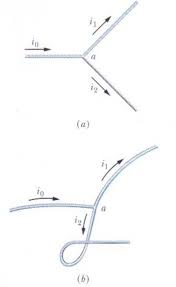
\includegraphics[scale=.7]{./imagens/26.jpg}
\end{center}

Se um condutor se bifurca em um nó a soma das correntes nos dois ramos é igual a corrente inicial:

\begin{equation}
    i_0=i_1+i_2
\end{equation}

A figura mostra parte de um circuito. Quais são o valor absoluto e o sentido da corrente i no fio da extremidade inferior direita?
\begin{center}
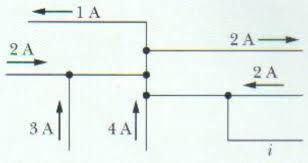
\includegraphics[scale=.7]{./imagens/27.jpg}
\end{center}

\subsection{Densidade de Corrente}

Podemos escrever a corrnte que atravessa o elemento de área como $\vec{J}\cdot d\vec{A}$, onde $d\vec{A}$ é o vetor área do elemento, perpendicular ao elemento. A corrente total que atravessa a superfície é, portanto,

\begin{equation}\label{18.23}
    i=\int \vec{J}\cdot d\vec{A}
\end{equation}

Se a corrente é uniforme em toda a superficie e paralela a $d\vec{A}$, $\vec{J}$ também é uniforme e paralela a $d\vec{A}$. Nesse caso, a \eqref{18.23} se torna

\begin{equation*}
    i=\int J dA= J\int dA = JA,
\end{equation*}

donde

\begin{equation}
    J=\dfrac{i}{A},
\end{equation}

em que $A$ é a área total da superfície.

Como a carga é conservada na transição, a quantidade de carga e a quantidade de corrente não podem mudar; o que muda é a densidade de corrente, que é maior no condutor mais estreito.

\begin{center}
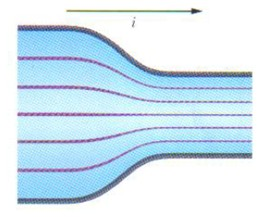
\includegraphics[scale=.7]{./imagens/28.jpg}
\end{center}

O espaçamento das linhas de corrente é inversamente proporcional à densidade de corrente; quanto mais próximas as linhas de corrente, mais a densidade de corrente.

Outra forma de encontrar a densidade de corrente é por

\begin{equation}
    \vec{J}=-\sigma \nabla\phi
\end{equation}

em que $\sigma$ é a resistividade do meio e $\phi$ é a função potencial do campo elétrico gerado pelas cargas.

VELOCIDADE DE DERIVA.

Velocidade de deriva (ou de arraste) é a velocidade com a qual as cargas se movem de maneira ordenada. Quando não está sendo percorrido por corrente, os elétrons de condução se movem aleatoriamente, sem que haja uma direção preferenicial. 

Considerando um pedaço de fio condutor de comprimento L e tomando n como o número de portadores por unidade de volume, podemos expressar a carga total q nesse pedaço de condutor, da seguinte forma:

%http://slideplayer.com.br/slide/10727011/

\begin{equation}
    \vec{J}=(ne)\vec{v}_d
\end{equation}


%http://www4.feb.unesp.br/dee/docentes/aquino/eletromag_I/eletromagI_teoria/cap06.pdf
\subsection{Resistência e Resistividade}

Medimos a resistência entre dois pontos de um condutor aplicando uma diferença de potencial $V$ entre esses pontos e medindo a corrente $i$ resultante. A resistência $R$ é dada por

\begin{equation}
    R=\dfrac{V}{i}
\end{equation}

Focando mais no material que no dispositivo, utilizaremos mais o Campo que a Diferença de potencial, mais a densidade de carga que a corrente. Utilizaremos a resistividade no lugar da resistência:

\begin{equation}
    \rho = \dfrac{E}{J}
\end{equation}

Compare essa equação com a anterior. A resistência está para a resistividade assim como a temperatura de um objeto está para seu calor específico.

CÁLCULO DA RESISTÊNCIA A PARTIR DA RESISTIVIDADE

VARIAÇÃO DA RESISTIVIDADE COM A TEMPERATURA

\subsection{Lei de Ohm}

A corrente que atravessa um dispositivo é sempre diretamente proporcional à diferença de potencial aplicada ao dispositivo. Um dispositivo obedece à essa lei se a sua resistência não depende do valor absoluto nem da polaridade da diferença de potencial aplicada. 


\subsection{Potência em Circuitos Elétricos}

A bateria fornece energia para os elétrons de condução, cujo movimento constitui a corrente.

De acordo com a lei de conservação da energia, a redução da energia potencial elétrica deve ser acompanhada por uma conversão da energia para outra forma qualquer. A potência $P$ associada a essa conversão pode ser expressa na forma

\begin{equation}
P=iV.
\end{equation}

\section{Circuitos}

\subsection{Trabalho, Energia e Força Eletromotriz}
Em um intervalo de tempo $dt$, uma carga $dq$ passa por todas as seçoes retas do circuito. A mesma carga entra no terminal de baixo potencial da fonte de tensão e sai do terminal de alto potencial. Para que a carga $dq$ se mova dessa forma, a fonte deve realizar sobre a carga um trabalho $dW$. Definimos a forma eletromotriz da fonte através do trabalho:

\begin{equation}\label{18.33}
    \varepsilon = \dfrac{dW}{dq}
\end{equation}

\subsection{Cálculo da Corrente em um Circuito de uma Malha}

\begin{equation}
    i=\dfrac{\varepsilon}{R}.
\end{equation}

\subsection{Circuitos com Mais de Uma Malha}

REGRA DOS NÓS

Quando uma diferença de potencial $V$ é aplicada a resistências ligadas em paralelo, todas as resistências são submetidas à mesma diferença de potencial. As resistências dessa categoria podem ser substituídas por uma resistência equivalente $R_{eq}$ com a mesma diferença de potencial $V$ e a mesma corrente total $i$ que as resistencias originais.

\begin{equation}
\dfrac{1}{R_{eq}}=\sum_{j=1}^n\dfrac{1}{R_j}
\end{equation}

No caso de duas resistêncas, a resistência equivalente é o produto das resistências dividido pela soma.

\subsection{Circuitos RC}

\subsubsection{Carga de um Capacitor}

\begin{equation}
    q=C\varepsilon(1-e^{-t/RC})
\end{equation}

\begin{equation}
    i=\dfrac{dq}{dt}=\left( \dfrac{\varepsilon}{R} \right)e^{-t/RC}
\end{equation}

\subsubsection{A Constante de Tempo}

O produto $RC$ aparece nas Eqs.

\subsubsection{Descarga de um Capacitor}

\section{Campos Magnéticos}
Podemos definir um campo magnético $\vec{B}$ como uma grandeza vetorial cuja direção conincide com aquela para a qual a força é zero. Depois de medir $\vec{F}_B$ para $\vec{v}$ perpendicular...

Podemos expressar esses resultados através da seguinte equação vetorial:

\begin{equation}\label{18.34}
    \vec{F_B}=q\vec{v}\times\vec{V}
\end{equation}

Significa que uma partícula com carga elétrica, $q$, movendo-se em um campo $\vec{B}$ com uma velocidade $\vec{v}$, experimenta uma força $\vec{F}$.

\subsection{Campos Cruzados: O Efeito Hall}

\begin{equation}
    n=\dfrac{Bi}{Vle}
\end{equation}

\subsection{Uma Partícula Carregada em Movimento Circular}

Página 198

\subsection{Força Magnética em um Fio Percorrido por Corrente}

\begin{equation}
    \vec{F_B}=i\vec{L}\times \vec{B}
\end{equation}

\subsection{O Momento Magnético Dipolar}

\begin{equation}
    \mu=NiA
\end{equation}

\begin{equation}
    \vec{\tau}=\vec{\mu}\times \vec{B}.
\end{equation}

\begin{equation}
    U(\theta)=-\vec{\mu}\times \vec{B}.
\end{equation}

\section{Campos Magnéticos Produzidos por Correntes}

O modulo do campo $d\vec{B}$ produzino no ponto $P$ por um elemento de corrente $id\vec{s}$ é dado por

\begin{equation}\label{18.10.1}
dB=\dfrac{\mu_0}{4\pi} \dfrac{i ds \sin \theta}{r^2}
\end{equation}

em que $\theta$ é o ângulo entre as direções de $d\vec{s}$ e $\vec{r}$, o vetor que liga $ds$ a $P$, e $\mu_0$é uma constante, conhecida como \textit{permeabilidade do vácuo}, cujo valor, por definição, é dado por

\begin{equation}
\mu_0=4\pi \times 10^{-7} T\cdot m/A \approx 1,26\times 10 ^{-6} T\cdot m/A
\end{equation}

A direção de $d\vec{B}$ é a do produto vetorial $d\vec{s}\times \vec{r}$. Podemos, portanto, escerver a equação \eqref{18.10.1} em forma vetorial, como

\begin{equation}\label{18.10.3}
dB=\dfrac{\mu_0}{4\pi} \dfrac{i d\vec{s}\times \vec{r}}{r^2} \mbox{ (lei de Biot-Savart)}.
\end{equation}

CAMPO MAGNÉTICO PRODUZIDO PELA CORRENTE EM UM FIO RETILÍNEO LONGO

%\begin{}




\section{Indução e Indutância}

\section{Oscilações Eletromagnéticas e Correntes Alternadas}

\section{Equações de Maxwell; Magnetismo da Matéria}

Serão apresentadas nas suas formas integrais e diferenciais.

\subsection{Primeira Lei}

Lei de Gauss para a eletricidade. Relaciona o fluxo elétrico às cargas elétricas envolvidas.
\begin{equation}
\begin{split}
    \oint{\vec{E}\cdot d\vec{A}}&=\frac{q}{\epsilon_0}\\
    \nabla\cdot E&=\frac{q}{\epsilon_0}
\end{split}
\end{equation}

\subsection{Segunda Lei}
Lei de Gauss para o magnetismo. Relaciona o fluxo magnético às cargas magnéticas envolvidas.

\begin{equation}
\begin{split}
    \oint{\vec{B}\cdot d\vec{A}}&=\frac{q}{\epsilon_0}\\
    \nabla\cdot B&=\frac{q}{\epsilon_0}
\end{split}
\end{equation}

\subsection{Terceira Lei}
Lei de Faradey. 

Relaciona o campo elétrico induzido à variação do fluxo magnético.

\begin{equation}
\begin{split}
\oint{\vec{E} \cdot d\vec{s}}&=-\dfrac{\partial \Phi_B}{\partial t}\\
\nabla \times \vec{E}&=-\dfrac{\partial B}{\partial t}
\end{split}   
\end{equation}


\subsection{Quarta Lei}
Lei de Ampère-Maxwell ou lei circuital de Ampère magnética. Relaciona o campo magnético induzido à variação do fluxo elétrico e à corrente.

\begin{equation}
\begin{split}
\oint{\vec{B} \cdot d\vec{s}}&=\mu_0\epsilon_0\dfrac{\partial \Phi_E}{\partial t}+\mu_0i\\
\nabla \times \vec{B}&=\mu_0\vec{J}+\dfrac{1}{c^2}\dfrac{\partial \vec{E}}{\partial t}
\end{split}   
\end{equation}

\subsection{Continuidade para cargas}

A densidade da corrente é o movimento de densidade de carga. A equação da continuidade diz que se a carga se move para fora de um volume diferencial (isto é, a divergência da densidade de corrente é positivo), então a quantidade de carga no interior desse volume vai diminuir, portanto, a taxa de variação da densidade de carga é negativa. Portanto, a equação da continuidade mostra que existe conservação da carga.
Em outras palavras, só poderia haver um fluxo de corrente se a quantidade de carga varia com o passar do tempo, já que está diminuindo ou aumentando em proporção à carga que é usada para alimentar tal corrente.
%\displaystyle
\begin{equation}
\nabla \cdot {\vec{J}}=-\dfrac{\partial \rho}{\partial t}
\end{equation}

Esta equação estabelece a conservação da carga.